\chapter{Experimental Results and Evaluation}
\section{Dataset Description}
The primary dataset is the project's controlled Windows VirtualBox image.
Its image states are recorded in the central evidence log: an initial
encrypted attempt, an unencrypted baseline, a version with eight known
files, a version with the ADS marker, and the subsequent slack working copy.
They are related states of one laboratory, not independent population
samples. The final working image's hash is recorded in Appendix B.

The baseline files include text, HTML, JSON, a Word document, a PDF, a JPEG,
and a PNG. Their known lengths range from 83 to 277,325 bytes. They provide
different file sizes and content formats, but the recovery routine does not
parse the internal document or image formats. Its question is whether the
selected NTFS stream is exported at the correct length. It would therefore
be misleading to treat these as eight independent format-decoder evaluations.

The hidden-data dataset contains a 36-byte resident ADS and a 25-byte marker
in document slack. Original marker expectations were recorded before the
later recovery checks. The final portable fixture additionally provides a
700-byte fragmented ordinary stream, a resident named stream, and a bounded
slack tail. The separate 50-sample campaign varies payload bytes and lengths
inside this small layout. All campaign inputs are constructed, and the
results should not be extrapolated to untested Windows allocation patterns.

\section{Laboratory Metadata and File Recovery}
Table \ref{tab:geometry} gives the geometry used for the historical raw-image
calculations. The earlier Windows \file{fsutil fsinfo ntfsinfo} comparison
supported the recorded fields; the command is documented as querying NTFS
volume information \cite{fsinfo}. This comparison is independent of the
parser's own arithmetic, although the underlying screenshots and logs remain
the evidence for what was actually observed.

\begin{table}[htbp]\centering
\caption{Recorded Windows laboratory geometry.}\label{tab:geometry}
\begin{tabular}{lr}\toprule
Property & Recorded value\\\midrule
Partition start LBA & 2,048\\
Partition byte offset & 1,048,576\\
Bytes per sector & 512\\
Bytes per cluster & 4,096\\
MFT record size in bytes & 1,024\\
MFT start LCN & 786,432\\
Absolute MFT byte offset & 3,222,274,048\\\bottomrule
\end{tabular}\end{table}

The November 15 result file records all eight recovered lengths matching
their expected values. Its original-content hash fields were unknown at
that time. On November 25, Jeff confirmed that the original SHA-256 hashes
match the recorded recovered hashes for all eight files. Table \ref{tab:files}
shows the current result. The original values in Appendix B are recorded
from this team confirmation; original command output was not attached.
This is a later comparison update, not a rerun or alteration of the
November 15 machine-generated report.

\begin{table}[htbp]\centering\small
\caption{Eight baseline files with matching lengths and team-confirmed hash matches.}
\label{tab:files}
\begin{tabular}{lrrl}\toprule
Filename & Record & Bytes & Original hash match\\\midrule
\file{Test.txt} & 38 & 83 & Match\\
\file{Test2.txt} & 39 & 1,778 & Match\\
\file{Testfile.docx} & 41 & 13,437 & Match\\
\file{SunflowerTest.jpg} & 42 & 48,647 & Match\\
\file{Thetestfile.pdf} & 43 & 17,247 & Match\\
\file{WaterfallTest.png} & 44 & 277,325 & Match\\
\file{HTMLtestdoc.html} & 55 & 608 & Match\\
\file{JSON_test_File.json} & 56 & 579 & Match\\\bottomrule
\end{tabular}\end{table}

\section{ADS and Slack Results}
The named resident stream \file{CapstoneEvidence} in record 58 produced
36 bytes matching the original marker hash. Its host's unnamed stream is
31 bytes, so selecting the default stream would answer a different question.
The named-stream identity is thus a necessary part of the result, not an
optional display label. Figure \ref{fig:adsproof} embeds the historical JSON
evidence rather than relying solely on a link.

\begin{figure}[p]\centering
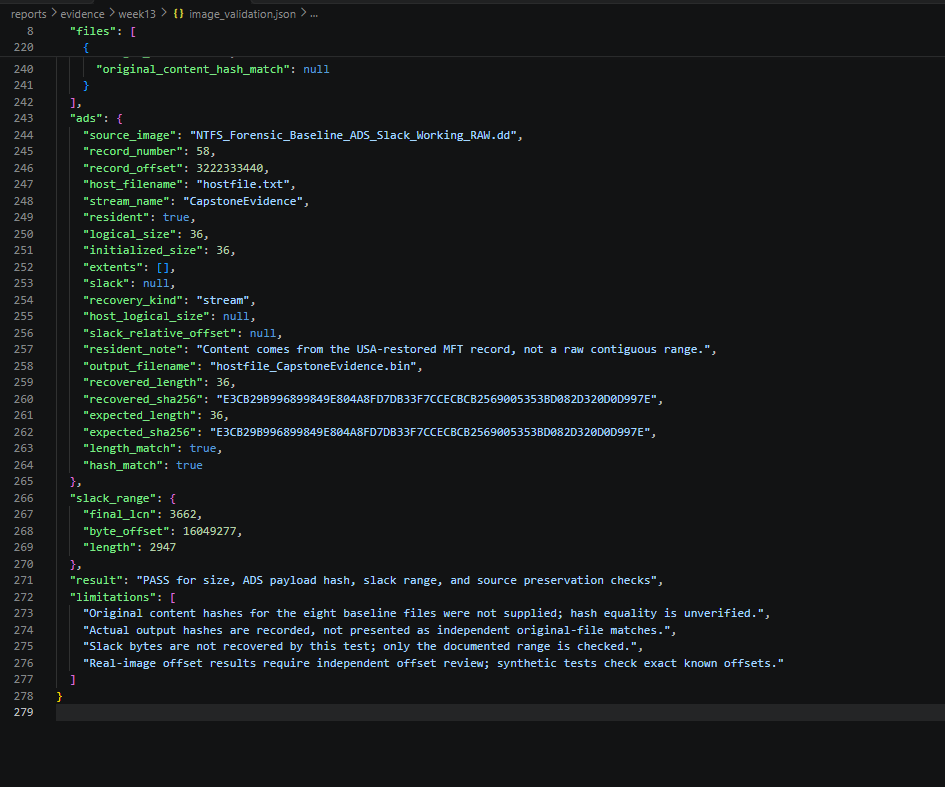
\includegraphics[width=\textwidth,height=6.8in,keepaspectratio]{w13_ads_validation.png}
\caption{Historical ADS validation evidence from November 15 showing the named stream and hash match.}
\label{fig:adsproof}\end{figure}

The document in record 41 had 13,437 logical bytes and 16,384 allocated bytes.
Its final content cluster left 2,947 slack bytes, beginning at absolute
offset 16,049,277, or hexadecimal \file{0x00F4E47D}. The requested 25-byte
marker was recovered with matching expected length and SHA-256.
Figure \ref{fig:slackproof} shows the bounded result, including the source
hash checks. The host document and slack payload are different exports.

\begin{figure}[p]\centering
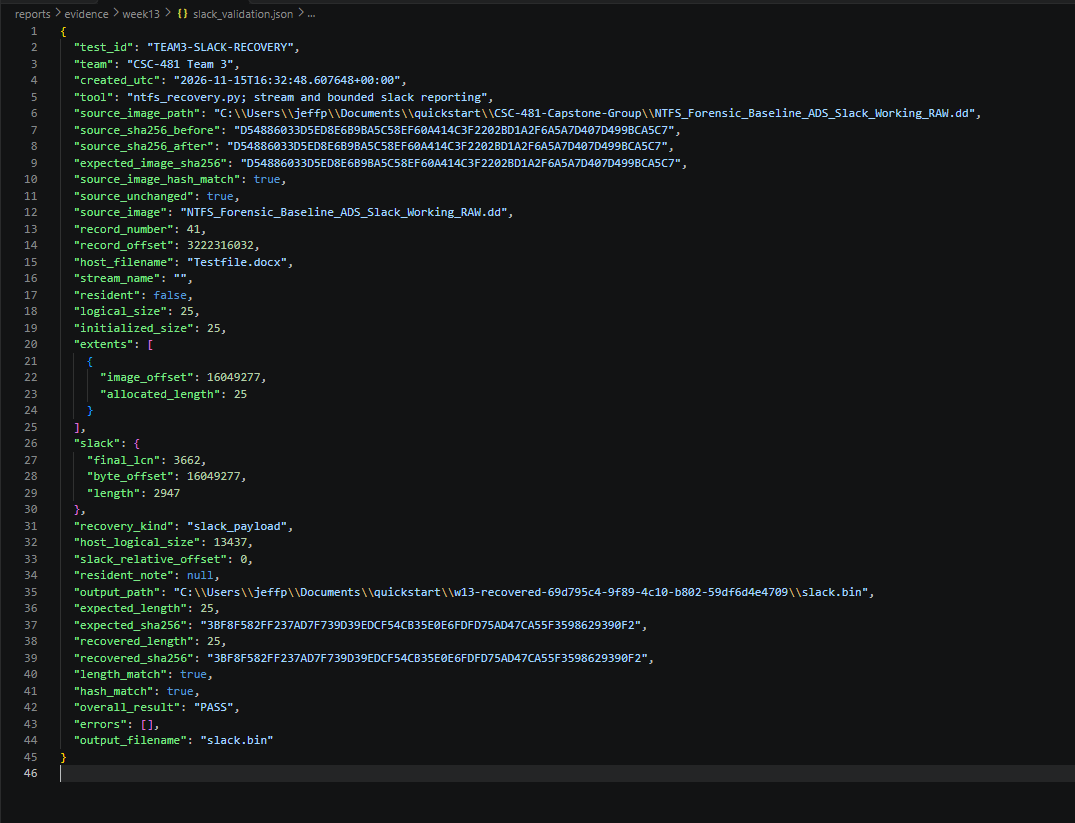
\includegraphics[width=\textwidth,height=6.8in,keepaspectratio]{w13_slack_validation.png}
\caption{Historical bounded-slack recovery evidence from November 15 with a 25-byte hash match.}
\label{fig:slackproof}\end{figure}

The working-image hash before and after the recorded recovery run was
identical. That observation supports preservation of the analyzed working
image during the run. It does not claim that the image equals the earlier
ADS-only source; the slack preparation intentionally changed its marker
range. The earlier full comparison records that preparation-stage difference.

\section{Capacity and Imperceptibility}
The measured Windows slack occupancy is 25/2,947 bytes, approximately
0.8483\%. Available capacity in that one tail is 2,947 bytes or 23,576 bits.
The ADS experiment demonstrates storage of 36 bytes or 288 bits; it does not
measure the maximum size of a named stream. These values describe filesystem
storage, so bits per pixel or audio sample would have no defined denominator.

No pixel or audio samples were modified, and no perceptual experiment was
performed. PSNR is therefore not applicable to the chosen carrier. The more
relevant preservation question is whether bytes outside the planned slack
range stayed the same and whether source images remained unchanged during
recovery. Historical full-copy comparison and image hashes provide evidence
for those questions. They do not constitute a human-perception or antivirus
evasion score.

\section{Synthetic Campaign and Robustness}
All 50 unchanged synthetic samples were recovered exactly and agreed with
the direct-byte-read baseline. All had zero bit errors. The five payload
sizes cover a one-byte minimum, the laboratory marker length, two intermediate
points, and the exact 324-byte synthetic tail boundary. Figure
\ref{fig:capacity} plots selected occupancy, while Table \ref{tab:campaign}
summarizes the paired clean and modified results.

\begin{table}[htbp]\centering
\caption{Synthetic campaign results with ten samples at each payload length.}
\label{tab:campaign}
\begin{tabular}{rrrrr}\toprule
Bytes & Occupancy \% & Exact clean & Changed hash failures & Changed BER \%\\\midrule
1 & 0.3086 & 10/10 & 10/10 & 12.5000\\
25 & 7.7160 & 10/10 & 10/10 & 0.5000\\
100 & 30.8642 & 10/10 & 10/10 & 0.1250\\
200 & 61.7284 & 10/10 & 10/10 & 0.0625\\
324 & 100.0000 & 10/10 & 10/10 & 0.0386\\\bottomrule
\end{tabular}\end{table}

\begin{figure}[htbp]\centering
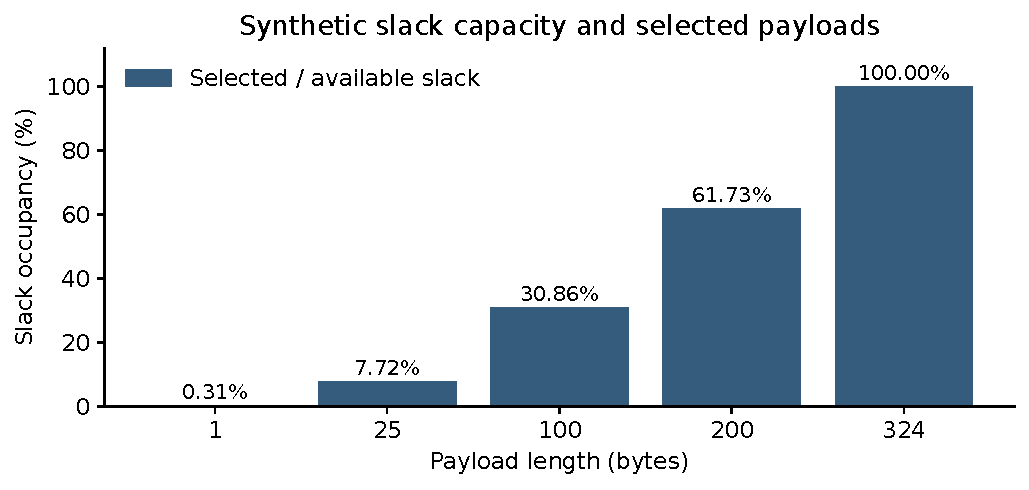
\includegraphics[width=0.94\textwidth]{capacity.pdf}
\caption{Payload occupancy in the 324-byte synthetic slack tail.}
\label{fig:capacity}\end{figure}

The deliberate one-bit changes were not corrected: the recovered bytes
contained exactly that one changed bit and the original-payload comparison
failed. Figure \ref{fig:ber} shows that the BER percentage falls as payload
length grows, even though every modified case contains the same number of
wrong bits. A small BER can therefore coexist with a decisive hash failure.
This is detection of corruption against a trusted expectation, not
steganographic recovery resilience after compression or file copying.

\begin{figure}[htbp]\centering
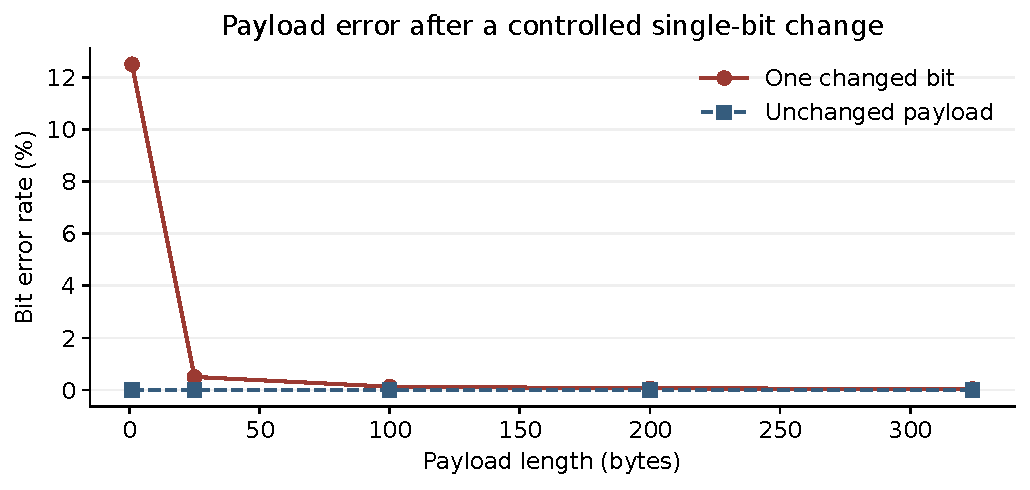
\includegraphics[width=0.94\textwidth]{ber.pdf}
\caption{Measured bit error rates after one deliberate stored-bit change.}
\label{fig:ber}\end{figure}

No corruption was introduced into the source used by each individual
recovery run. Modified images were created as separate inputs and given
their own correct expected image hash. This experimental control explains
why a modified case can have \file{source_unchanged=true} while its payload
hash fails: the source remained stable during recovery, but its payload no
longer matched the earlier original.

\section{Comparative Analysis}
The executed baseline seeks to the construction-known slack offset and
reads the specified length directly. It matched all 50 originals, as did
the structured recovery path. Their observed correctness difference on this
known-offset task is therefore zero percentage points. The structured tool's
additional behavior is metadata-based location, range validation, destination
protection, and saved verification; the baseline assumes location and length
are already correct.

That baseline is intentionally limited. It is not an independent NTFS parser
and does not validate the tool's behavior on unknown layouts. Nor is it a
performance comparison with The Sleuth Kit, Autopsy, Streams, or PhotoRec.
Timing columns are retained in the raw CSV, but single tiny cached reads
and a routine performing hashing, parsing, and report writes are not
equivalent workloads. We make no speed or scalability claim from them.

\section{Measured Detection and Evasion}
The separate November 25 detection experiment completed all 100 synthetic
cases. Table \ref{tab:detection} reports each fixed rule separately; the two
groups are not pooled into a general classifier score. Each group contains
25 intentionally hidden positives and 25 legitimate or ordinary negatives.

\begin{table}[htbp]\centering
\caption{Measured detection outcomes on constructed known-record inputs.}
\label{tab:detection}
\begin{tabular}{lrr}\toprule
Measure & ADS screening & Slack signature\\\midrule
True positives & 25 & 15\\
False negatives & 0 & 10\\
False positives & 10 & 0\\
True negatives & 15 & 25\\
Accuracy (\%) & 80 & 80\\
Detection rate (\%) & 100 & 60\\
False-positive rate (\%) & 40 & 0\\
Evasion rate (\%) & 0 & 40\\\bottomrule
\end{tabular}\end{table}

Named-stream screening detected all 25 deliberately hidden ADS cases.
It also flagged all ten legitimate named-stream controls; the 15 ordinary
files were not flagged. Thus stream presence is a useful review signal but
does not establish concealment intent. Its 40\% false-positive rate refers
to the hidden-content label, not an error locating the legitimate streams.

The slack rule detected all 15 plaintext markers, including placements at
varied offsets in the calculated tail. It missed all ten XOR-transformed
markers. All 25 negatives were correctly rejected, including ten with the
literal marker in logical file content rather than slack. The resulting
40\% evasion rate shows the fixed signature's dependence on unchanged bytes;
it does not show resistance to broader forensic inspection or other signatures.

\begin{figure}[htbp]\centering
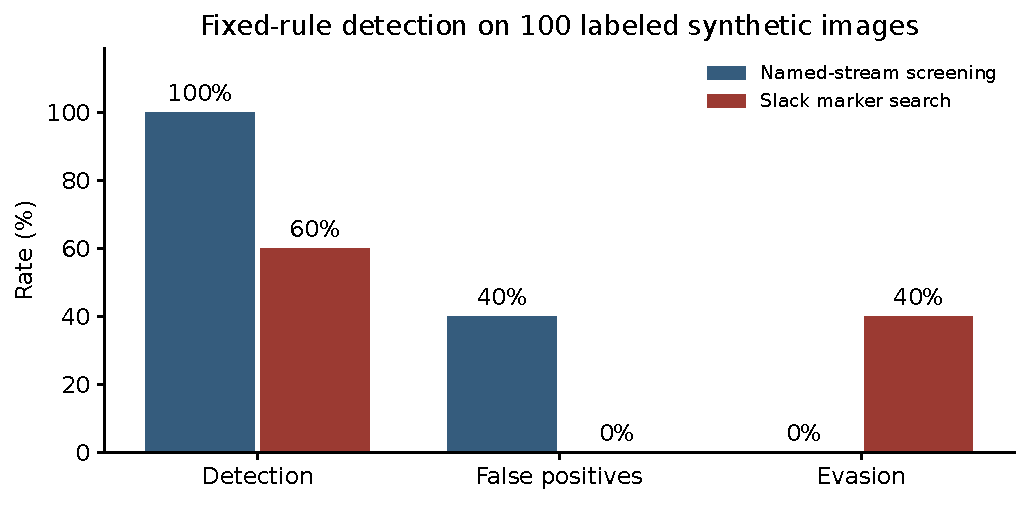
\includegraphics[width=0.94\textwidth]{detection.pdf}
\caption{Detection and evasion rates measured separately for two fixed rules.
Each rule was tested on 50 synthetic images.}
\label{fig:detection}\end{figure}

Both rules also flagged their known positives in the original Windows
working image: record 58 contained \file{CapstoneEvidence}, and record 41's
calculated slack contained the marker at relative offset zero. The image's
full SHA-256 matched the recorded expectation before and after screening.
All 100 synthetic image hashes were also unchanged. These two Windows
positives do not provide a real-volume false-positive estimate.

The fixed scenario proportions, shared metadata layout, known target records,
and known slack signature limit external validity. No rule was fitted or tuned
using the outcomes. The measured percentages describe this challenge set;
they are not estimates of hidden-content prevalence or detection accuracy
across arbitrary Windows volumes. Raw labels, decisions, hashes, and summary
are retained under \file{reports/evidence/final_detection/}.

\section{Regression Results and Evidence Limits}
The November 15 suite passed 64 tests in 4.729 seconds. The November 24
clean-copy release check passed 68 tests in 8.613 seconds, plus seven
acceptance checks. The four added tests cover deterministic data generation,
refusal of an existing dataset directory, end-to-end verification, and CLI
execution from an unrelated directory. Runtime differences cannot be
attributed to a performance regression because workload and execution
conditions differ.

The November 25 report extension passed all 73 tests in 9.567 seconds,
including five additional detection-campaign tests. This extends the current
report branch; it does not change the earlier tagged release's test count.

The strongest measured results are the two historical original-marker hash
matches and exact recovery in the constructed campaign. The team additionally
confirmed all eight baseline-file hash matches on November 25. Broad real-volume
coverage and realistic attack survival remain limited. The new labeled
detection experiment supplies rule-specific accuracy, false-positive, and
evasion measurements. General discovery of unknown hidden material remains
unvalidated. The results support controlled recovery and a bounded screening
comparison, rather than universal forensic discovery or covert security.
